\documentclass[presentation]{beamer}

\usepackage{tikz}
\usetikzlibrary{positioning,calc}
\usetikzlibrary{shapes.geometric}
\usetikzlibrary{backgrounds}% only to show the bounding box
\usetikzlibrary{shapes,arrows}
\usepackage{pgfplots}
\usepackage{pgfplotstable}
\usetikzlibrary{pgfplots.groupplots}
\pgfplotsset{compat=1.12}
\usepackage{appendixnumberbeamer}
\usepackage{amsmath}
\date{8th June 2016}
\usetheme{metropolis}

\pgfplotscreateplotcyclelist{decent cycle}{%
  {blue, mark=*, mark options={fill=blue},
    mark size=2pt},
  {cyan, mark=square*, mark options={fill=cyan},
    mark size=2pt},
  {magenta, mark=triangle*, mark options={fill=magenta},
    mark size=3pt},
  {blue, mark=*, mark options={fill=blue},
    mark size=2pt},
  {cyan, mark=square*, mark options={fill=cyan},
    mark size=2pt},
  {magenta, mark=triangle*, mark options={fill=magenta},
    mark size=3pt},
}

\pgfplotsset{
  decent/.style={
    cycle list name=decent cycle,
  }
}
\renewcommand{\vec}[1]{\ensuremath{\boldsymbol{#1}}}
\newcommand{\ddt}[1]{\frac{\partial #1}{\partial t}}
\newcommand{\zhat}{\hat{\vec{z}}}
\newcommand{\W}{\ensuremath{\mathbb{W}}}

\DeclareMathOperator{\grad}{grad}
\let\div\relax
\DeclareMathOperator{\div}{div}
\DeclareMathOperator{\curl}{curl}
\newcommand{\vsubset}[1]{\rotatebox[origin=c]{90}{\ensuremath{\subset}}}
\newcommand{\inner}[2]{\ensuremath{\langle #1, #2 \rangle}}
\author{Lawrence Mitchell\inst{1}}
\institute{
\inst{1}Departments of Computing and Mathematics, Imperial College
London
}

\graphicspath{{./\jobname.figures/}}

\newcommand{\arxivlink}[2]{%
  \href{http://www.arxiv.org/abs/#1}%
  {{\small\texttt{arXiv:\,#1\,[#2]}}}%
}
\newcommand{\doilink}[1]{%
  \href{http://dx.doi.org/#1}%
  {{\small\texttt{doi:\,#1}{}}}%
}
\usepackage[url=false,
            doi=true,
            isbn=false,
            style=authoryear,
            firstinits=true,
            uniquename=init,
            backend=biber]{biblatex}

\setbeamertemplate{bibliography item}{}
\renewcommand{\bibfont}{\footnotesize}
\addbibresource{references.bib}

\setlength{\bibitemsep}{1ex}

\renewbibmacro{in:}{}
\DeclareFieldFormat[article]{volume}{\textbf{#1}}
\DeclareFieldFormat{doi}{%
  doi\addcolon%
  {\scriptsize\ifhyperref{\href{http://dx.doi.org/#1}{\nolinkurl{#1}}}
    {\nolinkurl{#1}}}}
\AtEveryBibitem{%
\clearfield{pages}%
\clearfield{issue}%
\clearfield{number}%
}

\usepackage{minted}

\title{Firedrake: automating the finite element method by composing
  abstractions}

\begin{document}
\maketitle

\section{Introduction}

\begin{frame}
  \frametitle{Firedrake development team}
  \begin{itemize}
  \item[IC] David A.~Ham, Mikl\'os Homolya, Fabio Luporini, Gheorghe-Teodor
    Bercea, Paul H.~J.~Kelly
  \item[Bath] Andrew T.~T.~McRae
  \item[ECMWF] Florian Rathgeber
  \end{itemize}
  \begin{center}
    \url{www.firedrakeproject.org}
  \end{center}
\end{frame}

\begin{frame}[fragile]
  \frametitle{How do \emph{you} solve the Poisson equation?}
  \begin{columns}
    \begin{column}{0.65\textwidth}
\begin{minted}[fontsize=\tiny]{python}
from firedrake import *
mesh = UnitSquareMesh(100, 100)
V = FunctionSpace(mesh, "RT", 2)
Q = FunctionSpace(mesh, "DG", 1)
W = V*Q
u, p = TrialFunctions(W)
v, q = TestFunctions(W)

a = dot(u, v)*dx + div(v)*p*dx + div(u)*q*dx
L = -Constant(1)*v*dx
u = Function(W)
solve(a == L, u, solver_parameters={
    "ksp_type": "gmres", 
    "ksp_rtol": 1e-8,
    "pc_type": "fieldsplit",
    "pc_fieldsplit_type": "schur",
    "pc_fieldsplit_schur_fact_type": "full",
    "pc_fieldsplit_schur_precondition": "selfp",
    "fieldsplit_0_ksp_type": "preonly",
    "fieldsplit_0_pc_type": "ilu",
    "fieldsplit_1_ksp_type": "preonly",
    "fieldsplit_1_pc_type": "hypre"
})
\end{minted}
    \end{column}
    \hspace{-4em}
    \begin{column}{0.5\textwidth}
      Find $u\in V\times Q\subset H(\div)\times L^2$ s.t.
      \begin{align*}
        \inner{u}{v} + \inner{\div v}{p} &= 0 \quad\forall\, v \in V\\
        \inner{\div u}{q} &= -\inner{1}{q}\quad\forall\, q \in Q.
      \end{align*}
    \end{column}
  \end{columns}
\end{frame}


\begin{frame}
  How do we develop models?

  \begin{itemize}
  \item Choose equations
  \item Pick method/discretisation
  \item Decide on implementation language, target architecture
  \item Write code to implement method
  \item ...
  \item Change things, fix bits up.
  \end{itemize}
\end{frame}

\begin{frame}[fragile]
  \frametitle{FEM pseudocode}

  \begin{onlyenv}<1>
\begin{minted}[fontsize=\tiny]{python}
# x the input fields (e.g. current guess)
def form_residual(x):
    x_l <- x # global to ghosted
    for each element in mesh:
        x_e <- x_l[element] # gather through element map
        for each qp in element:
            basis_fns <- eval_basis_funs(qp)
            J <- compute_geometry(element, qp)
            for each bf in basis_fns:
                x_e_qp <- eval(x_e at qp)
                f_qp <- user_evaluation(qp, bf, x_e_qp)
            # insert into element residual
            f_e <- transform_to_physical(f_qp, J)
        f_l <- f_e # scatter through element map
    f <- f_l # ghosted to global
\end{minted}
  \end{onlyenv}

  \begin{onlyenv}<2>
\begin{minted}[fontsize=\tiny]{python}
                f_qp <- user_evaluation(qp, bf, x_e_qp)
\end{minted}
    \begin{itemize}
    \item Problem-specific variability in \emph{innermost} loop
    \item Efficient implementation may need to:
      \begin{itemize}
      \item vectorize across elements,
      \item vectorize within an element,
      \item exchange loop order,
      \item hoist loop-invariant code,
      \item exploit structure in basis functions,
      \item pre-evaluate geometry at quad points.
      \item Best choice will be architecture and
        problem/discretisation dependent.
      \end{itemize}
    \end{itemize}
  \end{onlyenv}
\end{frame}

\begin{frame}[standout]
  Say \emph{what}, not \emph{how}.
\end{frame}

\begin{frame}
  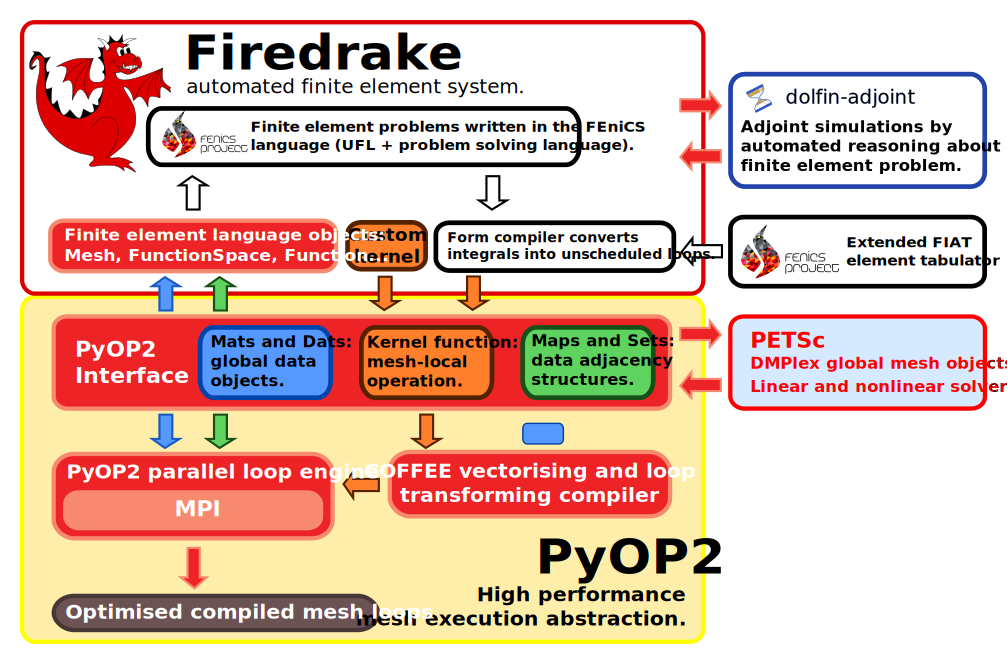
\includegraphics[width=\textwidth]{firedrake-stack}
\end{frame}

\section{Local kernels}

\begin{frame}
  \frametitle{Compiling variational forms}

  We use UFL \parencite{Alnaes:2014} from the FEniCS project for
  specifying variational problems.

  A \emph{form compiler} translates this to low-level executable code
  for evaluating the integral on an element.

\end{frame}

\begin{frame}[fragile]
  \frametitle{A simple example}
  \begin{columns}
    \begin{column}{0.5\textwidth}
\begin{minted}[fontsize=\tiny]{python}
mesh = UnitTriangleMesh()
V = FunctionSpace(mesh, "CG", 2)
u = TrialFunction(V)
v = TestFunction(V)
a = u*v*dx
\end{minted}
    \end{column}
\hspace{-3em}
    \begin{column}{0.65\textwidth}
\begin{minted}[fontsize=\tiny,mathescape]{c}
void integral(double A[6][6], 
    const double *restrict coords[6])
{
  double t0 = (-1 * coords[0][0]);
  double t1 = (-1 * coords[3][0]);
  /* $t2 \leftarrow |\det J|$ */
  double t2 = fabs(((t0 + (1 * coords[1][0])) *
                     (t1 + (1 * coords[5][0]))) +
                    (-1 * (t0 + (1 * coords[2][0])) *
                     (t1 + (1 * coords[4][0]))));
  static const double t3[6]     = {...};
  static const double t4[6][6]  = {...};
  for (int ip = 0; ip < 6; ip += 1) {
    double t5 = (t3[ip] * t2);
    for (int j = 0; j < 6; j += 1) {
      for (int k = 0; k < 6; k += 1) {
        A[j][k] += t5 * t4[ip][j] * t4[ip][k];
      }
    }
  }
}
\end{minted}
    \end{column}
  \end{columns}
\end{frame}
\begin{frame}[fragile]
  \frametitle{... and a complex one}
  \begin{onlyenv}<1>
\begin{minted}[fontsize=\tiny]{python}
mesh = UnitTriangleMesh()
V = VectorFunctionSpace(mesh, "CG", 2)
P = VectorFunctionSpace(mesh, "CG", 2)
v = TestFunction(V)
du = TrialFunction(V)  # Incremental displacement
u = Function(V)        # Displacement from previous iteration
B = Function(V)        # Body force per unit mass
# Kinematics
I = Identity(v.cell().topological_dimension())
F=I+grad(u)
C = F.T*F
E = (C - I)/2
E = variable(E)
# Material constants
mu = Constant(1.0)
lmbda = Constant(0.001)
# Strain energy function (material model) 
psi = lmbda/2*(tr(E)**2) + mu*tr(E*E)
S = diff(psi, E)       # Second Piola-Kirchhoff stress tensor
PK = F*S               # First Piola-Kirchoff stress tensor
# Variational problem
a = derivative((inner(PK, grad(v)) - inner(B, v))*dx, u, du)
\end{minted}
  \end{onlyenv}
  \begin{onlyenv}<2>
{\fontsize{3pt}{4pt}\selectfont
\begin{columns}
\begin{column}{0.5\textwidth}
\begin{minted}{c}
void integral(double A[12][12], const double *restrict coords[6],
              const double *restrict w_0[12],
              const double w_1[1],
              const double w_2[1])
{
  double t0 = (-1 * coords[0][0]);
  double t1 = (t0 + (1 * coords[1][0]));
  double t2 = (-1 * coords[3][0]);
  double t3 = (t2 + (1 * coords[5][0]));
  double t4 = (t0 + (1 * coords[2][0]));
  double t5 = (t2 + (1 * coords[4][0]));
  double t6 = ((t1 * t3) + (-1 * t4 * t5));
  double t7 = fabs(t6);
  static const double t8[6]  = {...};
  double t9 = (w_2[0] / 2);
  double t10 = (1 * 1);
  double t11 = (2 * t10);
  double t12 = (-1 * 1);
  double t13 = (t1 / t6);
  double t14 = ((-1 * t4) / t6);
  double t15 = ((-1 * t5) / t6);
  double t16 = (t3 / t6);
  static const double t17[6][12] = {...};
  static const double  t18[6][12]  = {...};
  static const double  t19[6][12]  = {...};
  static const double  t20[6][12]  = {...};
  for (int  ip  = 0; ip < 6; ip += 1) {
    double  t59[12] ;
    double  t60[12] ;
    double  t65[12] ;
    double  t66[12] ;
    double  t24  = 0.0;
    double  t23  = 0.0;
    double  t22  = 0.0;
    double  t21  = 0.0;
    for (int  i_0  = 0; i_0 < 12; i_0 += 1) {
      t21 += t20[ip][i_0] * w_0[i_0][0];
      t22 += t19[ip][i_0] * w_0[i_0][0];
      t23 += t18[ip][i_0] * w_0[i_0][0];
      t24 += t17[ip][i_0] * w_0[i_0][0];
    }
    double  t25  = (1 + (t16 * t24) + (t15 * t23));
    double  t26  = ((t14 * t24) + (t13 * t23));
    double  t27  = ((t16 * t22) + (t15 * t21));
    double  t28  = (1 + (t14 * t22) + (t13 * t21));
    double  t29  = (t10 * (((t25 * t26) + (t27 * t28)) / 2));
    double  t30  = ((t29 + t29) * w_1[0]);
    double  t31  = ((t12 + (t25 * t25) + (t27 * t27)) / 2);
    double  t32  = ((t12 + (t26 * t26) + (t28 * t28)) / 2);
    double  t33  = (t11 * (t31 + t32) * t9);
    double  t34  = (t10 * t31);
\end{minted}
\end{column}
\begin{column}{0.5\textwidth}
\begin{minted}{c}
    double  t35  = (t33 + ((t34 + t34) * w_1[0]));
    double  t36  = (t10 * t32);
    double  t37  = (t33 + ((t36 + t36) * w_1[0]));
    double  t38  = (t10 * (((t26 * t25) + (t28 * t27)) / 2));
    double  t39  = ((t38 + t38) * w_1[0]);
    for (int  k  = 0; k < 12; k += 1) {
      double  t40  = ((t16 * t19[ip][k]) + (t15 * t20[ip][k]));
      double  t41  = ((t14 * t17[ip][k]) + (t13 * t18[ip][k]));
      double  t42  = (t41 * t25);
      double  t43  = ((t16 * t17[ip][k]) + (t15 * t18[ip][k]));
      double  t44  = (t43 * t26);
      double  t45  = ((t14 * t19[ip][k]) + (t13 * t20[ip][k]));
      double  t46  = (t45 * t27);
      double  t47  = (t40 * t28);
      double  t48  = (t10 * ((t42 + t44 + t46 + t47) / 2));
      double  t49  = ((t48 + t48) * w_1[0]);
      double  t50  = (t43 * t25);
      double  t51  = (t40 * t27);
      double  t52  = ((t50 + t50 + t51 + t51) / 2);
      double  t53  = (t41 * t26);
      double  t54  = (t45 * t28);
      double  t55  = ((t53 + t53 + t54 + t54) / 2);
      double  t56  = (t11 * (t52 + t55) * t9);
      double  t57  = (t10 * t55);
      double  t58  = (t56 + ((t57 + t57) * w_1[0]));
      t59[k] = (t40 * t39) + (t49 * t27) + (t45 * t37) + (t58 * t28);
      t60[k] = (t43 * t39) + (t49 * t25) + (t41 * t37) + (t58 * t26);
      double  t61  = (t10 * t52);
      double  t62  = (t56 + ((t61 + t61) * w_1[0]));
      double  t63  = (t10 * ((t44 + t42 + t47 + t46) / 2));
      double  t64  = ((t63 + t63) * w_1[0]);
      t65[k] = (t40 * t35) + (t62 * t27) + (t45 * t30) + (t64 * t28);
      t66[k] = (t43 * t35) + (t62 * t25) + (t41 * t30) + (t64 * t26);
    }
    double  t67  = (t8[ip] * t7);
    for (int  j  = 0; j < 12; j += 1) {
      double  t68  = ((t14 * t19[ip][j]) + (t13 * t20[ip][j]));
      double  t69  = ((t14 * t17[ip][j]) + (t13 * t18[ip][j]));
      double  t70  = ((t16 * t19[ip][j]) + (t15 * t20[ip][j]));
      double  t71  = ((t16 * t17[ip][j]) + (t15 * t18[ip][j]));
      for (int  k  = 0; k < 12; k += 1) {
        A[j][k] += t67 * ((t66[k] * t71) + (t65[k] * t70) +
                          (t60[k] * t69) + (t59[k] * t68));
      }
    }
  }
}
\end{minted}
\end{column}
\end{columns}
}
  \end{onlyenv}
\end{frame}

\begin{frame}
  \frametitle{Two-stage form compilation}
  \begin{enumerate}[<+->]
  \item Lower finite element expressions to tensor-algebra
  \item Lower tensor algebra to unscheduled loop nest of scalar
    expressions.
  \item Apply optimisation passes to minimise operation count, make
    code amenable to vectorising compilers.
  \end{enumerate}

\end{frame}
\begin{frame}
  \frametitle{Lowering FE}
  \begin{equation*}
    c_q = \sum_r \mathcal{E}_{q, r} c_r
  \end{equation*}
  $\mathcal{E}_{q, r}$ provided by FIAT as tabulation of 2D array.
  \begin{block}<2->{Structure in $\mathcal{E}$}
    \begin{equation*}
      \mathcal{E}_{q,r} = \mathcal{E}_{(q_x,r_x),(q_y, r_y)}
    \end{equation*}
    But $\mathcal{E}$ factorises
    \begin{equation*}
      \mathcal{E}_{q, r} = \mathcal{E}^x_{q_x, r_x}
      \mathcal{E}^y_{q_y, r_y}
    \end{equation*}
    WIP: exploiting structure for automated sum-factorisation.
  \end{block}
\end{frame}

\begin{frame}[fragile]
  \frametitle{Optimisation of finite element kernels}
  
  \begin{problem}
    Modern optimising compilers do a bad job on finite element
    kernels.
  \end{problem}
  \begin{exampleblock}{Code motion (or not)}
\begin{minted}[fontsize=\tiny]{c}
for (i = 0; i < L; i++ )
   for (j = 0; j < M; j++)
      for (k = 0; k < N; k++)
         A[j][k] += f(i, j)*g(i, k)
\end{minted}
  \end{exampleblock}
  \begin{corollary}
    We need to spoon-feed the compiler already optimised code.
  \end{corollary}
\end{frame}
\begin{frame}
  \frametitle{COFFEE}
  The cause of, and solution to, all of life's problems.
  No single optimal scheduling of loop nests that occur in finite
  element integration.  Depends on degree, form complexity, basis
  function structure.

  By generating code and passing to a special-purpose optimising
  compiler, we are able to achieve significant reductions in operation
  counts.  Mostly through judicious use of loop-invariant code motion
  and CSE.

%   empirical:
  
% \begin{minted}[fontsize=\tiny]{python}
% for i in ...:
%    for j in ...:
%       for k in ...:
%           A[j, k] += f(i, k)*g(i, j) + ...
% \end{minted}

% General purpose compilers will hoist \verb~g(i, j)~, but not \verb~f(i, k)~.
  \begin{center}
    \url{github.com/coneoproject/COFFEE}\\
    \cite{Luporini:2015} \doilink{10.1145/2687415}
    \cite{Luporini:2016} \arxivlink{1604.05872}{cs.MS}\\
  \end{center}
\end{frame}
\section{Global iteration}

\begin{frame}[fragile]
  \frametitle{PyOP2}
  A library for expressing data parallel iterations
\begin{description}
\item[{\emph{Sets}}] iterable entities
\item[{\emph{Dats}}] abstract managed arrays (data defined on a set)
\item[{\emph{Maps}}] relationships between elements of sets
\item[{\emph{Kernels}}] the "local" computation
\item[{\emph{par\_loop}}] Data parallel iteration over a set
\end{description}
Arguments to parallel loop indicate how to gather/scatter global
data using \emph{access descriptors}

\begin{minted}[fontsize=\tiny]{python}
par\_loop(kernel, iterset, data1(map1, READ), data2(map2, WRITE))
\end{minted}
\begin{center}
  \url{github.com/OP2/PyOP2}\\
  \cite{Rathgeber:2012} \doilink{10.1109/SC.Companion.2012.134}
\end{center}
\end{frame}

\begin{frame}
  \frametitle{Optimising mesh iteration}
  We all know we \emph{ought} to do loop tiling
  \begin{itemize}
  \item Better data reuse/locality
  \item Can hide communication latency
  \end{itemize}
  But it's very invasive to an application (especially an unstructured
  one).

  PyOP2 approach makes it possible to provide loop tiling in a
  semi-automated way within the library.

  Application code does ``whatever'', PyOP2 sees a sequence of
  parallel loops with data dependencies.  Can tile over multiple
  loops.
\end{frame}


\section{Symbolic computation}

\begin{frame}
  \frametitle{Maintaining symbolic information}
  Firedrake uses UFL \cite{Alnaes:2014} to specify problems

  Can perform AD at a high level, resulting in efficient code for
  adjoints, etc...

  Can produce matrix-free with low-order preconditioners
  ``automatically''.  Symbolic reasoning and composition of solvers,
  rather than just algebraic manipulation (all that is available with
  assembled matrices).
  Allows symbolically, rather than just algebraically, expressing
  complex solvers (WIP, with Rob Kirby (Baylor)).
\end{frame}



\begin{frame}
  \frametitle{Mesh iteration}
  Mesh-based solvers execute \emph{local} operation over mesh
  gathering data with some \emph{stencil}.

  PyOP2 captures these iterations and manages the execution.

  Most naive implementation just does ``the iteration you would have
  written''.

  But, we can do more.  In particular, unstructured mesh loop-tiling.
\end{frame}

\begin{frame}
  \frametitle{Solvers}
  
\end{frame}

\begin{frame}
  \frametitle{Applications of Firedrake}
  \begin{itemize}
  \item Colin Cotter (Imperial College).  3D mimetic finite element
    dynamical core for NWP
  \item Onno Bokhove (University of Leeds). Freak waves,
    fluid-structure interactions (boats in waves).
  \item Justin Chang (University of Houston).  Positivity preserving
    methods for advection-diffusion-reaction geochemical systems
  \item Tuomas K\"arn\"a (Oregon Health and Science). 3D coastal and
    estuarine ocean modelling
  \item Andrew McRae, Chris Budd (University of Bath).  $r-$adaptivity
    on the sphere.
  \item Francis Poulin (University of Waterloo).  Stability of jets
    and vortices in the ocean.
  \end{itemize}
\end{frame}
\appendix
\begin{frame}[allowframebreaks]
  \frametitle{References}
  \printbibliography[heading=none]
\end{frame}
\end{document}
